% ##################################################################################################################
\chapter{Belgium: The Use of MATSim Within an Estimation Framework for Assessing Economic Impacts of River Floods}
\label{ch:belgium}
\hfill \textbf{Author:} Ismaïl Saadi, Jacques Teller, Mario Cools

% ##################################################################################################################
\section{Problem Statement}
In the context of past river floods in Belgium, and given the significant probability that such events take place in the near future, the need to assess both the potential direct and indirect economic impact is essential to enable the formulation of an adequate policy program and efficient flood risk management. 
In this regard, it is proposed to assess the flood risk  at the micro-scale level (\ie individual buildings for exposure analysis and direct economic damage estimation, individual companies for indirect economic damage estimation, 10\,meter grid spacing for land-use modeling, and individuals/vehicles for transportation models). 
To this end, an integrated modeling framework combining different simulation theories from a multidisciplinary perspective is being developed. 
Figure~\ref{fig:belgium_fig1} describes the followed procedure to measure the annual flood risk. 
A more detailed description of the whole modeling chain is available in \citet[][]{DewalsEtAl_IAHR_2015}.

 % ------------
\createfigure%
{Economic impact estimation procedure}%
{Economic impact estimation procedure}%
{\label{fig:belgium_fig1}}%
{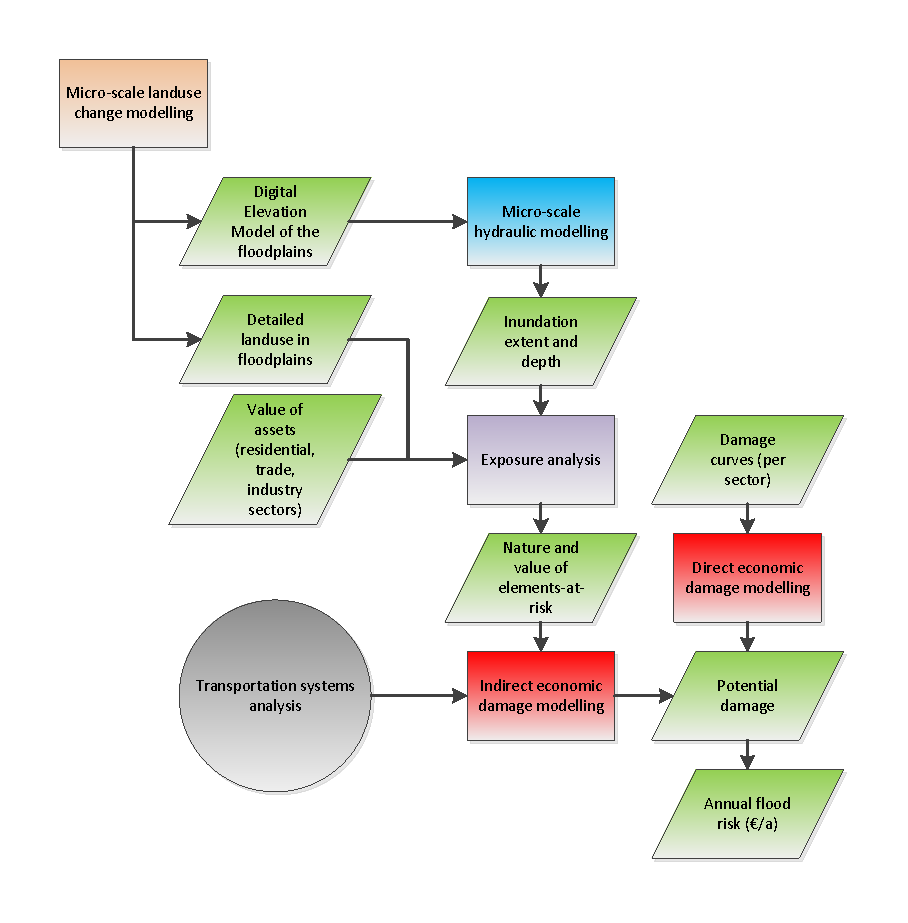
\includegraphics[width=0.97\textwidth, angle=0]{scenarios/figures/belgium_fig1.pdf}}%
{}
% ------------

A basic premise in the modeling framework is that different families of spatial patterns might influence the damage intensity caused by river floods (\eg land use change, transportation systems). 
In this chapter, we focus on how \gls{matsim} is being integrated within this overall framework, and thus focus on the \gls{tsa} within the overall estimation procedure. With respect to this \gls{tsa}, two configurations are distinguished: a freight and passenger model. 
Regarding the passenger model, a \gls{matsim} scenario is developed at the national scale to simulate the travel demand at a base year (2010) and its evolution during the following years. 
Recall that the main objective is to study the effects of river floods on the transportation network and consequently on travel demand; both of them from an economical point of view. 
Besides a freight travel demand model has been developed, to enable the interactions between passenger and good flows. 
It has to be acknowledged that at the current state of development this is still an aggregate four-step model, but development is ongoing to develop also an agent-based model for the freight side.  

% ##################################################################################################################
\section{Data Collection}
As inputs, \gls{matsim} requires a synthetic population (or travel demand) file as well as its related transportation network. 
Concerning the first input, no recent census is available unfortunately. 
The latest dates from~2001. 
In this context, a synthetic population is derived from more recent travel surveys \citep[e.g.,][]{CornelisEtAl_ResRep_BELDAM_2012} by employing a Gibbs sampler \citep[][]{FarooqBierlaireHurtubiaEtAl2013Simulationbasedpopulation}. 
The Belgian National Household Travel Survey \citep[e.g.,][]{CornelisEtAl_ResRep_BELDAM_2012} contains socio-demographics and activity travel diaries with a detailed description of activity start, end times and durations. 
Activity locations are also available but at the municipality code. level. They are generally referred by using the new municipalities referencing system: \gls{lau} level~2. 
With respect to the transportation network, the \gls{osm} network data has been used.

% ##################################################################################################################
\section{Inputs Preparation}
% ========================================================================================
\subsection{Network}
The network data of Belgium, downloaded in~2015, is available online from the \gls{osm} server. 
It consists of 100\,467 nodes and 232\,715 links. 
Network quality is generally acceptable according to many \gls{matsim} users even if manual adjusting is suitable for specific links.

% ========================================================================================
\subsection{Synthetic Population}
The preparation of a synthetic population presents a great challenge for the current case study. 
In practice, only micro-data are available to enable the synthesizing of a population. 
From these partial views of the true population, the use of a Gibbs sampler enables the (re-)construction of the joint distribution. 
The outputs seem to be encouraging when comparing the computed predictions with the reference dataset. 
Here, we propose to test the methodology by synthesizing some relevant variables for both transportation and urban systems simulations at the household level (see Figure~\ref{fig:belgium_fig2}).

 % ------------
\createfigure%
{Examples of households synthesized attributes}%
{Examples of households synthesized attributes}%
{\label{fig:belgium_fig2}}%
{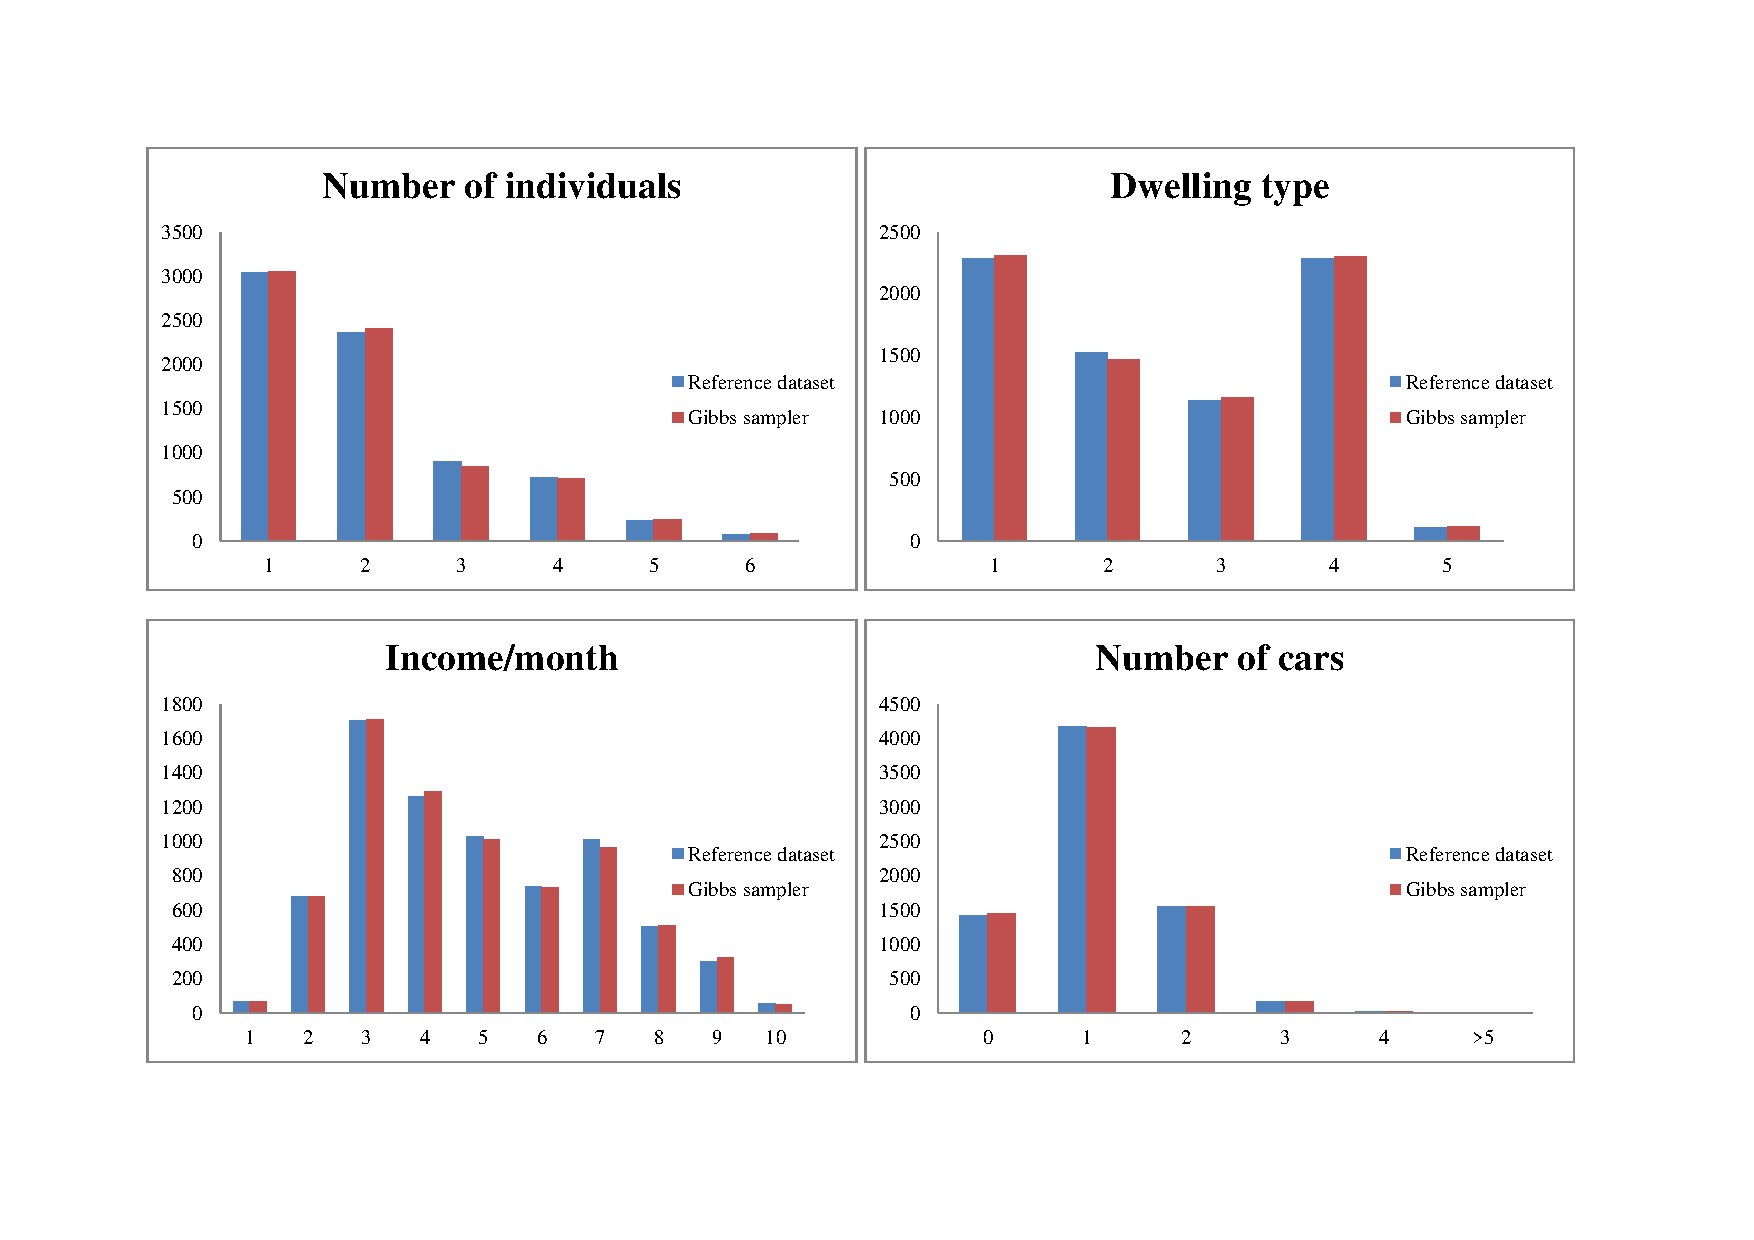
\includegraphics[width=0.97\textwidth, angle=0]{scenarios/figures/belgium_fig2.pdf}}%
{}
% ------------

% ========================================================================================
\subsection{Activity-Based Pattern Generation}
Consequently, after the synthetic population has been generated, \emph{activity types}, \emph{activity times} and \emph{activity locations} are generated and associated to the agents using an activity-based pattern generator. 
Using a combined set of machine learning techniques, daily activity planers are generated for each agent. 
As shown in Figure~\ref{fig:belgium_fig3}, the model suggests some promising preliminary results. The activity-pattern generator is calibrated by using micro-data such as activity travel diaries extracted from travel surveys. 
The calibration quality will be measured after analyzing the outputs of \gls{matsim} scenario when traffic counts will be compared. 
If the comparison between observed and simulated traffic counts suggests a significant deviation, a direct approach based on traffic counts \citep[][]{CoolsEtAl_TRR_2010} could be opportune to adjust the parameters of the activity-based pattern generator.

 % ------------
\createfigure%
{Activity chains generation}%
{Activity chains generation}%
{\label{fig:belgium_fig3}}%
{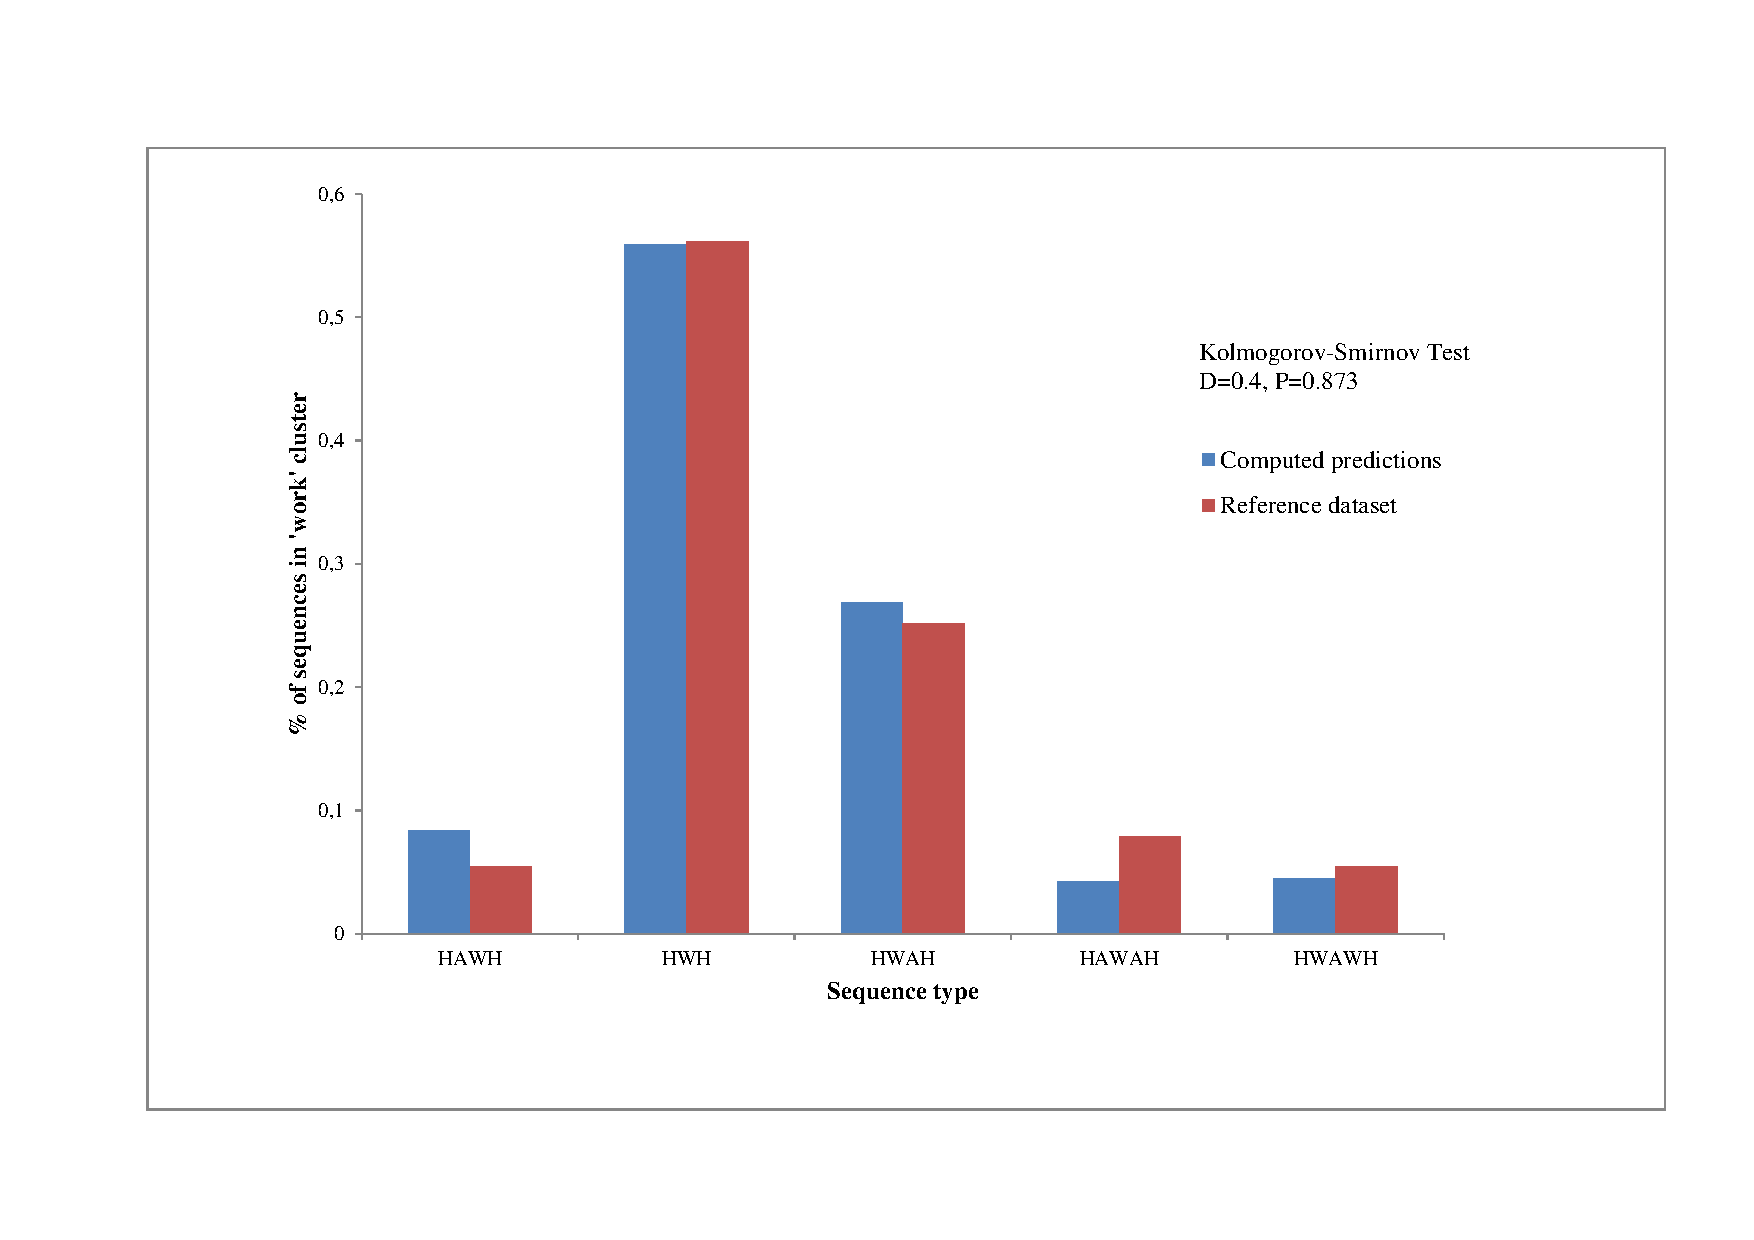
\includegraphics[width=0.97\textwidth, angle=0]{scenarios/figures/belgium_fig3.pdf}}%
{}
% ------------

As outlined by \citet[][]{CoolsEtAl_TRB_2011}, uncertainties introduced by the statistical distributions of the random components existing in most of activity-based models might be significant. 
In this regard, some key indicators (\eg proportions of sequences type) will be investigated to measure the impact of micro-simulation error.

% ##################################################################################################################
\section{General Modeling Framework}
In Saadi et al. (2014), the overall modeling framework is presented as well as the integration of the components in the scheme. 
This paper includes all the concepts that will probably be used to build the future \gls{matsim} scenario. 
Figure~\ref{fig:belgium_fig4} is a partial view of the overall modeling framework on which researches are in progress at the moment.

 % ------------
\createfigure%
{Partial Modeling Framework}%
{Partial Modeling Framework}%
{\label{fig:belgium_fig4}}%
{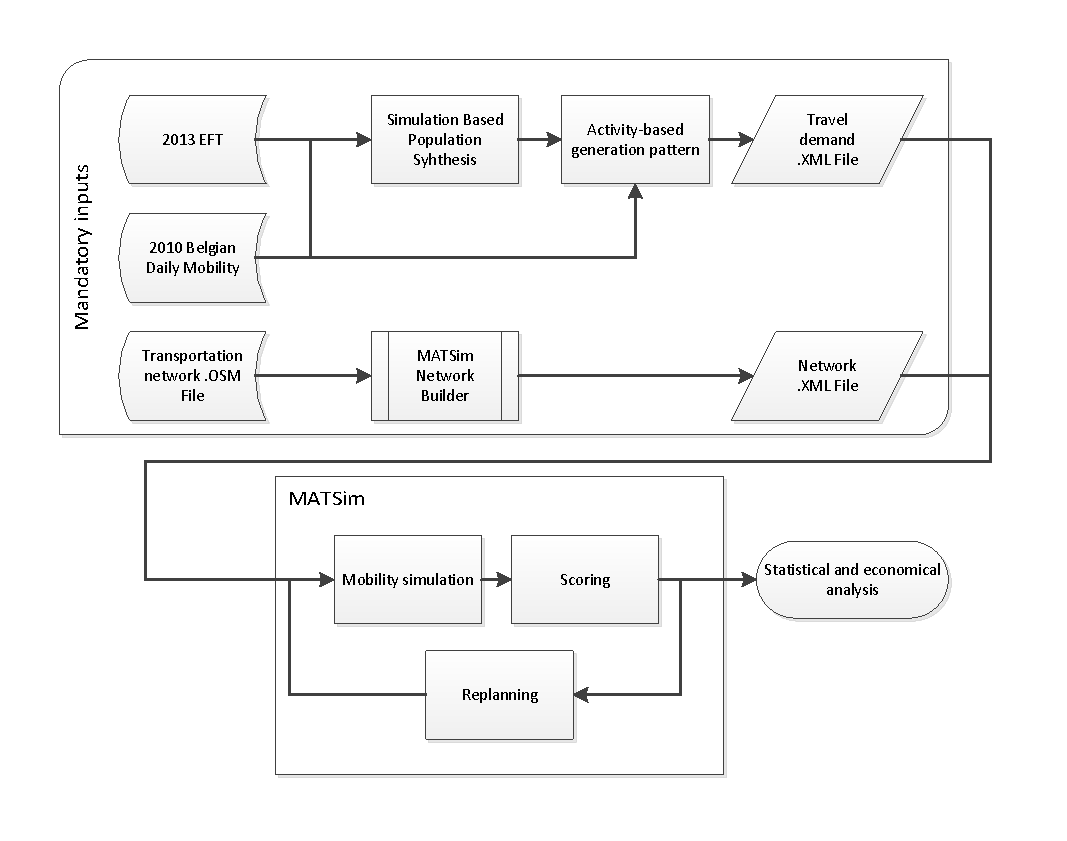
\includegraphics[width=0.97\textwidth, angle=0]{scenarios/figures/belgium_fig4.pdf}}%
{}
% ------------

% ##################################################################################################################
\section{Modeling Network Disruption}
As mentioned previously, this study also suggests modeling the network inaccessibility occurring after river floods. 
This approach assumes that the links capacities subjected to river floods are reduced depending on floods intensity. 
Given the fact that the damage is mainly a function of the water depth, the idea is to intersect a steady-state inundation map with the transportation network or, at least, the area concerned by floods \citep[][]{SaadiEtAl_ICTTE_2014}. 
Then, an extension of the analysis will be realized by including time series of river floods to enable a better understanding of the dynamic effects (\eg response to river floods propagation, return way and time to the new equilibrium point between transport supply and demand). 
A similar problem had been studied to simulate an evacuation scenario due to a tsunami in the city of Padang \citep[][]{LaemmelGretherNagel2009TimeDependentNetworks} (Section~\ref{ch:padang}. 
This work is interesting in terms of network dynamic evolution during the simulation of the scenario.

% ##################################################################################################################
\section{Next Development Steps}
When the complete integrated agent-based transportation model is ready, the coupling with the land-use change \gls{ca} based model proposed by \citet[][]{MustafaEtAl_PES_2014} will be achieved to allow more interactions between those two patterns. 
This connection will be the basis for an innovative micro-scale \gls{luti} model.
In this context, more accurate predictions about future river floods influenced by the different micro-scale patterns will be carried out.

% ##################################################################################################################







